 \let\negmedspace\undefined
\let\negthickspace\undefined
\documentclass[journal]{IEEEtran}
\usepackage[a5paper, margin=10mm, onecolumn]{geometry}
%\usepackage{lmodern} % Ensure lmodern is loaded for pdflatex
\usepackage{tfrupee} % Include tfrupee package

\setlength{\headheight}{1cm} % Set the height of the header box
\setlength{\headsep}{0mm}     % Set the distance between the header box and the top of the text

\usepackage{gvv-book}
\usepackage{gvv}
\usepackage{cite}
\usepackage{amsmath,amssymb,amsfonts,amsthm}
\usepackage{algorithmic}
\usepackage{graphicx}
\usepackage{textcomp}
\usepackage{xcolor}
\usepackage{txfonts}
\usepackage{listings}
\usepackage{enumitem}
\usepackage{mathtools}
\usepackage{gensymb}
\usepackage{comment}
\usepackage[breaklinks=true]{hyperref}
\usepackage{tkz-euclide} 
\usepackage{listings}
% \usepackage{gvv}                                        
\def\inputGnumericTable{}                                 
\usepackage[latin1]{inputenc}                                
\usepackage{color}                                            
\usepackage{array}                                            
\usepackage{longtable}                                       
\usepackage{calc}                                             
\usepackage{multirow}                                         
\usepackage{hhline}                                           
\usepackage{ifthen}                                           
\usepackage{lscape}
\usepackage{circuitikz}


\renewcommand{\thefigure}{\theenumi}
\renewcommand{\thetable}{\theenumi}
\setlength{\intextsep}{10pt} % Space between text and floats


\numberwithin{equation}{enumi}
\numberwithin{figure}{enumi}
\renewcommand{\thetable}{\theenumi}


% Marks the beginning of the document
\begin{document}
\bibliographystyle{IEEEtran}
\vspace{3cm}

\title{GATE 2022}
\author{EE25BTECH11060 - Namaswi Vajjala}
\maketitle

% (add your content here)
\noindent \textbf{Q. 1 -- Q. \textbf{5}} carry one mark each.

\begin{enumerate}
\item After playing  \underline{\hspace{2cm}} hours of tennis,I am feeling \underline{\hspace{2cm}} tired to walk back
\hfill{(GATE ME 2022)}
\begin{multicols}{2}
    \begin{enumerate}
        \item too/too
        \item too/two
        \item two/two
        \item two/too
    \end{enumerate}
\end{multicols}
\item  The average of the monthly salaries of M, N and S is \rupee 4000. The average of the monthly salaries of N, S and P is \rupee 5000. The monthly salary of P is \rupee 6000.What is the monthly salary of M as a percentage of the monthly salary of P? 
\hfill{(GATE ME 2022)}
\begin{multicols}{4}
    \begin{enumerate}
        \item 50 \%
        \item 75\%
        \item  100\%
        \item  125\%
    \end{enumerate}
\end{multicols}
\item A person travelled 80 km in 6 hours. If the person travelled the first part with a uniform speed of 10 kmph and the remaining part with a uniform speed of 18kmph.What percentage of the total distance is travelled at a uniform speed of 10 kmph?
\hfill{(GATE ME 2022)}
\begin{multicols}{4}
    \begin{enumerate}
        \item 28.25
        \item 37.25
        \item 43.75
        \item 50.00
    \end{enumerate}
\end{multicols}
 \item Four girls P, Q, R and S are studying languages in a University. P is learning French and Dutch. Q is learning Chinese and Japanese. R is learning Spanish and French. S is learning Dutch and Japanese.Given that: French is easier than Dutch; Chinese is harder than Japanese; Dutch is easier than Japanese, and Spanish is easier than French.Based on the above information, which girl is learning the most difficult pair of languages?
 \hfill{(GATE ME 2022)}
\begin{multicols}{4}
    \begin{enumerate}
        \item P
        \item Q
        \item  R
        \item  S
    \end{enumerate}
\end{multicols}

\item A block with a trapezoidal cross-section is placed over a block with rectangular cross section as shown above. Which one of the following is the correct drawing of the view of the 3D object as viewed in the direction indicated by an arrow in the above figure?
 \begin{figure}[H]
    \centering
    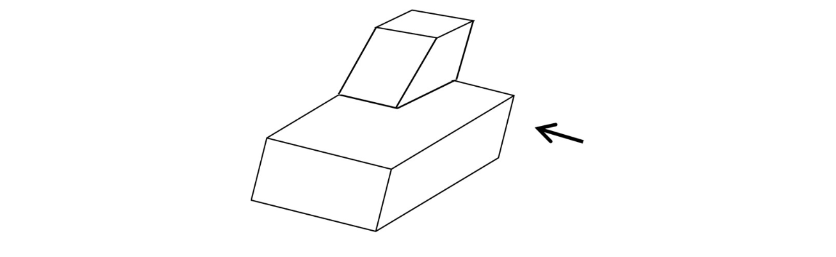
\includegraphics[width = 0.6\columnwidth]{figs/fig4.1.png}
    \caption*{}
    \label{fig:Q5}
    \end{figure}
    \hfill{(GATE ME 2022)}
\begin{enumerate} 
\item \begin{figure}[H]
    \centering
    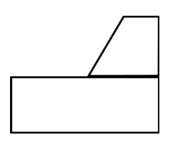
\includegraphics[width = 0.5\columnwidth]{figs/fig4.2.png}
    \caption*{}
    \label{fig:Q5}
    \end{figure}
\item \begin{figure}[H]
    \centering
    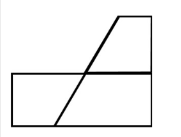
\includegraphics[width = 0.5\columnwidth]{figs/fig4.3.png}
    \caption*{}
    \label{fig:Q5}
    \end{figure}
\item \begin{figure}[H]
    \centering
    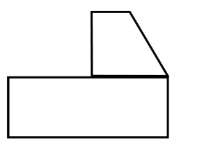
\includegraphics[width = 0.5\columnwidth]{figs/fig4.4.png}
    \caption*{}
    \label{fig:Q5}
    \end{figure}

\item \begin{figure}[H]
    \centering
    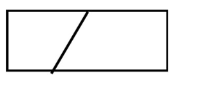
\includegraphics[width = 0.5\columnwidth]{figs/fig4.5.png}
    \caption*{}
    \label{fig:Q5}
    \end{figure}
   \end{enumerate} 

\item Humans are naturally compassionate and honest. In a study using strategically placed wallets that appear "lost", it was found that wallets with money are more likely to be returned than wallets without money. Similarly, wallets that had a key and money are more likely to be returned than wallets with the same amount of money alone. This suggests that the primary reason for this behavior is compassion and empathy. Which one of the following is the CORRECT logical inference based on the information in the above passage?
\hfill{(GATE ME 2022)}
\begin{enumerate}   
\item Wallets with a key are more likely to be returned because people do not care about money
\item Wallets with a key are more likely to be returned because people relate to suffering of others
\item Wallets used in experiments are more likely to be returned than wallets that are really lost
\item Money is always more important than keys
\end{enumerate}
\item A rhombus is formed by joining the midpoints of the sides of a unit square.What is the diameter of the largest circle that can be inscribed within the rhombus?
\hfill{(GATE ME 2022)}
\begin{multicols}{4}
    \begin{enumerate}
        \item $\frac{1}{\sqrt{2}}$
        \item $\frac{1}{\sqrt{2}}$
        \item $\sqrt{2}$
        \item $2\sqrt{2}$
    \end{enumerate}
\end{multicols}

\item An equilateral triangle, a square and a circle have equal areas.
What is the ratio of the perimeters of the equilateral triangle to square to circle?
\hfill{(GATE ME 2022)}
\begin{enumerate}
    \item \( 3\sqrt{3} : 2 : \sqrt{\pi} \)
    \item \( \sqrt{(3 \sqrt{3})} : 2 : \sqrt{\pi} \)
    \item \( \sqrt{(3 \sqrt{3})} : 4 : 2\sqrt{\pi} \)
    \item \( \sqrt{(3 \sqrt{3})} : 2 : 2\sqrt{\pi} \)
\end{enumerate}
\item Given below are three conclusions drawn based on the following three
statements.
Statement 1: All teachers are professors.
Statement 2: No professor is a male.
Statement 3: Some males are engineers.
Conclusion I: No engineer is a professor.
Conclusion II: Some engineers are professors.
Conclusion III: No male is a teacher.
Which one of the following options can be logically inferred?
\hfill{(GATE ME 2022)}
\begin{enumerate}
    \item Only conclusion III is correct
\item Only conclusion I and conclusion II are correct
\item Only conclusion II and conclusion III are correct
\item only conclusion I and conclusion III are correct
\end{enumerate}

\item In a 12-hour clock that runs correctly, how many times do the second, minute,and hour hands of the clock coincide, in a 12-hour duration from 3 PM in a day to 3 AM the next day?
\hfill{(GATE ME 2022)}
\begin{multicols}{4}
\begin{enumerate}
    \item 11
    \item 12
    \item 144
    \item 2
\end{enumerate}
\end{multicols}
\item The limit
\begin{align*}
p = \lim_{x \to \pi} \left(\frac{x^2 + \alpha x + 2\pi^2}{x - \pi + 2 \sin x}\right)
\end{align*}
has a finite value for a real \(\alpha\). The value of \(\alpha\) and the corresponding limit \(p\) are
\hfill{(GATE ME 2022)}
\begin{enumerate}
    \item \(\alpha = -3\pi,\) and \(p = \pi\)
    \item \(\alpha = -2\pi,\) and \(p = 2\pi\)
    \item \(\alpha = \pi,\) and \(p = \pi\)
    \item \(\alpha = 2\pi,\) and \(p = 3\pi\)
\end{enumerate}

\item Solution of \(\nabla^2 T = 0\) in a square domain \((0 < x < 1 \text{ and } 0 < y < 1)\) with boundary conditions:
\begin{align*}
 T(x,0) = x; \quad T(0,y) = y; \quad T(x,1) = 1 + x; \quad T(1,y) = 1 + y   
\end{align*}
\begin{enumerate}
    \item T$\brak{x,y} = x - xy + y$
    \item  T$\brak{x,y} = x + y$
    \item T$\brak{x,y} = -x+y$
    \item T$\brak{x,y} =x+xy+y$
\end{enumerate}
\hfill{(GATE ME 2022)}
\item Given a function 
\[
\varphi = \frac{1}{2}(x^2 + y^2 + z^2)
\]
in three-dimensional Cartesian space, the value of the surface integral
\begin{align*}
\iint_{S} \mathbf{\hat{n}} \cdot \nabla \varphi \, dS,
\end{align*}
where \( S \) is the surface of a sphere of unit radius and \( \mathbf{\hat{n}} \) is the outward unit normal vector on \( S \), is
\hfill{(GATE ME 2022)}
\begin{multicols}{4}
\begin{enumerate}
    \item$ 4\pi$
\item  $3\pi$  
\item $\frac{4\pi}{3}$ 
\item 0
\end{enumerate}
\end{multicols}

\item The Fourier series expansion of $x^3$ in the interval $-1 \le x < 1$ with periodic continuation has
\hfill{(GATE ME 2022)}
\begin{enumerate}
    \item only sine terms

\item only cosine terms

\item both sine and cosine terms

\item only sine terms and a non-zero constant
\end{enumerate}
\item If \(\mathbf{A} = \begin{bmatrix}
10 & 2k + 5 \\
3k - 3 & k + 5
\end{bmatrix}\) is a symmetric matrix, the value of \(k\) is  
\begin{multicols}{4}
\begin{enumerate}
    \item 8
    \item 5
    \item -0.4
    \item $\dfrac{1 + \sqrt{1561}}{12}$
\end{enumerate}
\end{multicols}
\item A uniform light slender beam AB of section modulus EI is pinned by a frictionless joint A to the ground and supported by a light inextensible cable CB to hang a weight W as shown. If the maximum value of W to avoid buckling of the beam AB is obtained as A $\pi^2 $ EI, where $\pi$ is the ratio of circumference to diameter of a circle,
then the value of $\beta$ is
\begin{figure}[H]
    \centering
    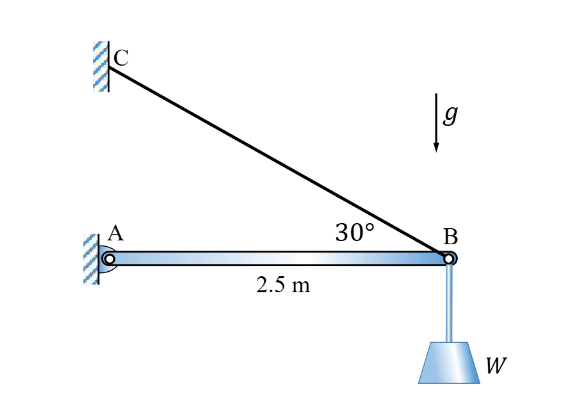
\includegraphics[width = 0.5\columnwidth]{figs/fig4.6.png}
    \caption*{}
    \label{fig:Q16}
    \end{figure}

\begin{multicols}{4}
    \begin{enumerate}
        \item 0.0924 $m^(-2)$
        \item 0.0713  $m^(-2)$
        \item 0.1261 $m^(-2)$
        \item 0.1417 $m^(-2)$
    \end{enumerate}
\end{multicols}

 \item The figure shows a schematic of a simple Watt governor mechanism with the
spindle $o_1 o_2$ rotating at an angular velocity o about a vertical axis. The balls at P and S have equal mass. Assume that there is no friction anywhere and all other components are massless and rigid. The vertical distance between the horizontal plane of rotation of the balls and the pivot O1 is denoted by h. The value of h = 400 mm at a certain $\omega$. If is doubled, the value of h will be
\begin{figure}[H]
    \centering
    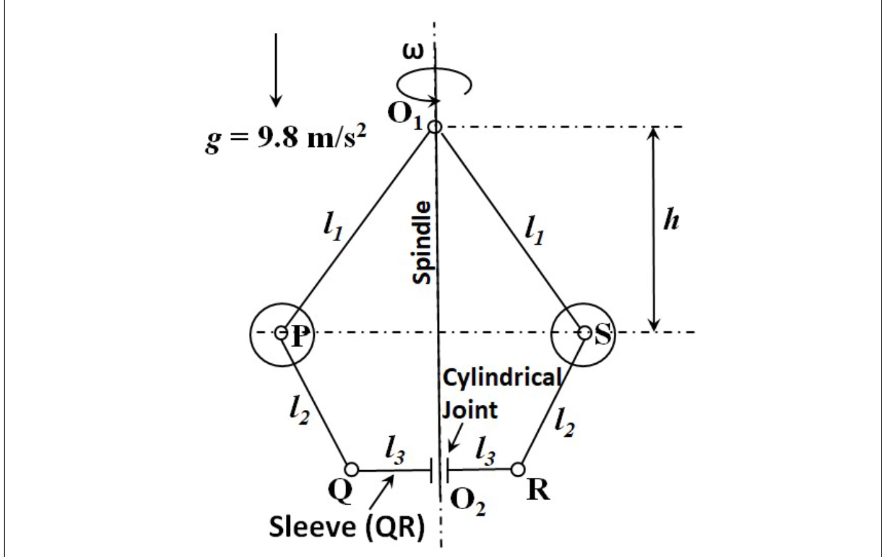
\includegraphics[width = 0.5\columnwidth]{figs/fig4.7.png}
    \caption*{}
    \label{fig:Q17}
    \end{figure}
    \hfill{(GATE ME 2022)}
\begin{multicols}{4}
    \begin{enumerate}
        \item 50
        \item 100
        \item 150
        \item 200
    \end{enumerate}
\end{multicols}
\item A square threaded screw is used to lift a load W by applying a force F. Efficiency of square threaded screw is expressed as
\hfill{(GATE ME 2022)}
\begin{enumerate}
    \item The ratio of work done by W per revolution to work done by F per revolution
    \item $\frac{W}{F}$
    \item $\frac{F}{W}$
    \item The ratio of work done by F per revolution to work done by W per revolution
\end{enumerate}
 
\item 
A CNC worktable is driven in a linear direction by a lead screw connected directly to a stepper motor. The pitch of the lead screw is 5 mm. The stepper motor completes one full revolution upon receiving 600 pulses. If the worktable speed is 5 m/minute and there is no missed pulse, then the pulse rate being received by the stepper motor is
\hfill{(GATE ME 2022)}
 \begin{multicols}{4}
     \begin{enumerate}
         \item 20
         \item 10
         \item 3
         \item 15
     \end{enumerate}
 \end{multicols}

\item The type of fit between a mating shaft of diameter 25.0-0.010 mm and a hole of+ 0.015 diameter 25.015-0.015 mm is
\hfill{(GATE ME 2022)}
\begin{multicols}{4}
    \begin{enumerate}
        \item Clearance
  \item Transition
\item Interference
\item Linear
\end{enumerate}
\end{multicols}

\item In a linear programming problem, if a resource is not fully utilized, the shadow price of that resource is
\hfill{(GATE ME 2022)}
\begin{multicols}{4}
    \begin{enumerate}
        \item positive
        \item negative
        \item zero
        \item infinity
    \end{enumerate}
\end{multicols}

\item Which one of the following is NOT a form of inventory?
\hfill{(GATE ME 2022)}
\begin{multicols}{2}
    \begin{enumerate}
        \item Raw materials
\item Work-in-process materials
\item Finished goods
\item CNC Milling Machines
    \end{enumerate}
\end{multicols}
\item 
The Clausius inequality holds good for
\hfill{(GATE ME 2022)}
\begin{multicols}{2}
    \begin{enumerate}
        \item any process
        \item any cycle
        \item only reversible process
        \item only reversible cycle
    \end{enumerate}
\end{multicols}
  \item A tiny temperature probe is fully immersed in a flowing fluid and is moving with zero relative velocity with respect to the fluid. The velocity field in the fluid is 
    \[
    \vec{V} = 2x\, \hat{\imath} + (y + 3t)\, \hat{\jmath},
    \]
    and the temperature field in the fluid is 
    \[
    T = 2x^2 + xy + 4t,
    \]
    where \(x\) and \(y\) are the spatial coordinates, and \(t\) is the time. The time rate of change of temperature recorded by the probe at ...

(x=1, y =1, t =1) is
\hfill{(GATE ME 2022)}
\begin{multicols}{4}
    \begin{enumerate}
        \item 4
        \item 0
        \item 8
        \item 14
    \end{enumerate}
\end{multicols}

\item In the following two-dimensional momentum equation for natural convection over a surface immersed in a quiescent fluid at temperature \( T_\infty \) 
(\( g \) is the gravitational acceleration, \( \beta \) is the volumetric thermal expansion coefficient, \( \nu \) is the kinematic viscosity, 
\( u \) and \( v \) are the velocities in \( x \) and \( y \) directions, respectively, and \( T \) is the temperature)

\begin{align*}
u \frac{\partial u}{\partial x} + v \frac{\partial u}{\partial y} 
= g \beta (T - T_\infty) + \nu \frac{\partial^2 u}{\partial y^2},
\end{align*}

the term \( g \beta (T - T_\infty) \) represents
\hfill{(GATE ME 2022)}
\begin{enumerate}

\item 
Ratio of inertial force to viscous force. 
\item
Ratio of buoyancy force to viscous force. 
\item
Viscous force per unit mass. 
\item Buoyancy force per unit mass
\end{enumerate}

\item Assuming the material considered in each statement is homogeneous, isotropic, linear
elastic, and the deformations are in the elastic range, which one or more of the
following statement(s) is/are TRUE?
\hfill{(GATE ME 2022)}
\begin{enumerate}
    \item 
A body subjected to hydrostatic pressure has no shear stress.
\item 
If a long solid steel rod is subjected to tensile load, then its volume increases.
\item 
Maximum shear stress theory is suitable for failure analysis of brittle materials.
\item 
If a portion of a beam has zero shear force, then the corresponding portion of the
elastic curve of the beam is always straight.
\end{enumerate}
\item 
Which of the following heat treatment processes is/are used for surface hardening
of steels?
\hfill{(GATE ME 2022)}
\begin{enumerate}
    \item carburinizing
    \item cyaniding
    \item annealing
    \item carbonitriding
\end{enumerate}

\item Which of the following additive manufacturing technique(s) can use a wire as a feedstock material?
\hfill{(GATE ME 2022)}
\begin{enumerate}
    \item Stereolithography
\item Fused deposition modeling
\item Selective laser sintering
\item Directed energy deposition processes
\end{enumerate}

\item 
Which of the following methods can improve the fatigue strength of a circular mild teel (MS) shaft?
\hfill{(GATE ME 2022)}
\begin{enumerate}
    \item Enhancing surface finish
\item hot peening of the shaft
\item Increasing relative humidity
\item Decreasing relative humidity
\end{enumerate}
\item The figure shows a purely convergent nozzle with a steady, inviscid compressible flow of an ideal gas with constant thermophysical properties operating under choked condition. The exit plane shown in the figure is located within the nozzle. If the inlet pressure (Po) is increased while keeping the back pressure (Pback)
unchanged, which of the following statements is/are true?

\begin{figure}[H]
    \centering
    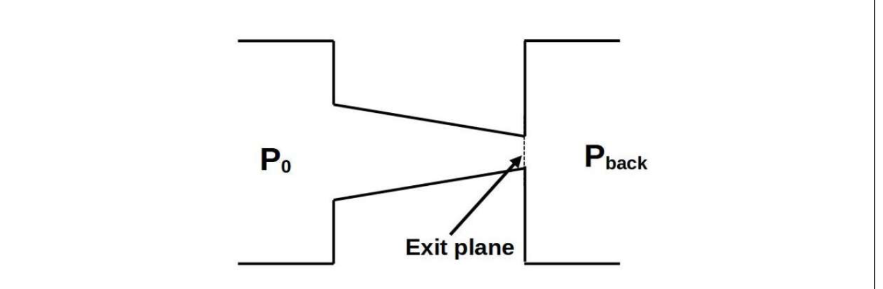
\includegraphics[width = 0.5\columnwidth]{figs/fig4.8.png}
    \caption*{}
    \label{fig:Q30}
    \end{figure}
\hfill{(GATE ME 2022)}
 \begin{enumerate}
     \item Mass flow rate through the nozzle will remain unchanged.
\item Mach number at the exit plane of the nozzle will remain unchanged at unity.
\item Mass flow rate through the nozzle will increase.
\item Mach number at the exit plane of the nozzle will become more than unity.
 \end{enumerate}
\item 
The plane of the figure represents a horizontal plane. A thin rigid rod at rest is pivoted without friction about a fixed vertical axis passing through O. Its mass moment of inertia is equal to 0.1 kg.cm2 about O. A point mass of 0.001 kg hits it normally at 200 cm/s at the location shown, and sticks to it. Immediately after the impact, the angular velocity of the rod is
rad/s (in integer).
 \begin{figure}[H]
    \centering
    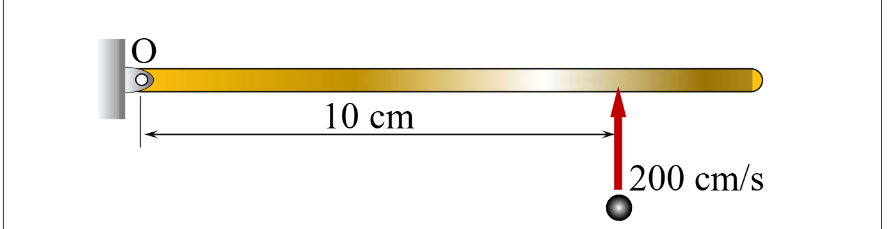
\includegraphics[width = 0.5\columnwidth]{figs/fig4.9.png}
    \caption*{}
    \label{fig:Q31}
    \end{figure}
 \hfill{(GATE ME 2022)}
\item 
A rigid uniform annular disc is pivoted on a knife edge A in a uniform gravitational field as shown, such that it can execute small amplitude simple harmonic motion in the plane of the figure without slip at the pivot point. The inner radius r and outer radius R are such that $r^2 = R^2/2$, and the acceleration due to gravity is g. If the time period of small amplitude simple harmonic motion is given by T =  $\beta \pi \sqrt{(R/g)}$ where $\pi$ is the ratio of circumference to diameter of a circle, then $\beta$ =
(round off to 2 decimal places).
\begin{figure}[H]
    \centering
    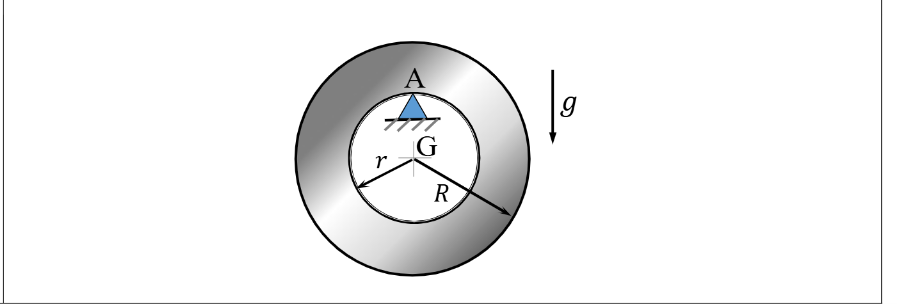
\includegraphics[width = 0.5\columnwidth]{figs/fig4.10.png}
    \caption*{}
    \label{fig:Q32}
    \end{figure}
\hfill{(GATE ME 2022)}
\item  Electrochemical machining operations are performed with tungsten as the tool, and copper and aluminum as two different workpiece materials. Properties of copper and aluminum are given in the table below.

\begin{center}
\begin{tabular}{|>{\bfseries}m{3cm}|m{3cm}|m{3cm}|m{3cm}|}
\hline
Material & Atomic mass (amu) & Valency & Density (g/cm\textsuperscript{3}) \\
\hline
Copper & 63 & 2 & 9 \\
\hline
Aluminum & 27 & 3 & 2.7 \\
\hline
\end{tabular}
\end{center}
Ignore overpotentials, and assume that current efficiency is 100\% for both the workpiece materials. Under identical conditions, if the material removal rate (MRR) of copper is 100 mg/s, the MRR of aluminum will be \underline{\hspace{4cm}} mg/s \textit{(round-off to two decimal places)}.

\item absolute value of the work done during the process is
decimal places).
A polytropic process is carried out from an initial pressure of 110 kPa and volume
of 5 $m^3$ to a final volume of 2.5 $m^3$. The polytropic index is given by n = 1.2. The
kJ (round off to 2
places)
\hfill{(GATE ME 2022)}
\item 
A flat plate made of cast iron is exposed to a solar flux of 600 W/m2 at an ambient
temperature of 25 \degree C. Assume that the entire solar flux is absorbed by the plate.

Cast iron has a low temperature absorptivity of 0.21. Use Stefan-Boltzmann
constant = 5.669 x$ 10^{-8 }W/m^2-K^4$. Neglect all other modes of heat transfer except
radiation.

Under the aforementioned conditions, the radiation equilibrium temperature of the
C (round off to the nearest integer).
\textbf{Q.36-Q.65 carry two marks each}
\item The value of the integral
\begin{align*}
    \oint \left( \frac{6z}{2z^4 - 3z^3 + 7z^2 - 3z + 5} \right) \, dz
\end{align*}
evaluated over a counter-clockwise circular contour in the complex plane enclosing only the pole $z = i$, where $i$ is the imaginary unit, is
\hfill{(GATE ME 2022)}
\begin{enumerate}
     \item $(-1 + i)\pi$
    \item  $(1 + i)\pi$
    \item $2(1 - i)\pi$
    \item$(2 + i)\pi$
    
\end{enumerate}
\item An L-shaped elastic member ABC with slender arms AB and BC of uniform cross-section is clamped at end A and connected to a pin at end C. The pin remains in continuous contact with and is constrained to move in a smooth horizontal slot. The section modulus of the member is same in both the arms. The end C is subjected to a horizontal force P and all the deflections are in the plane of the figure. Given the length AB is 4a and length BC is a, the magnitude and direction of the normal force on the pin from the slot, respectively, are
\begin{figure}[H]
    \centering
    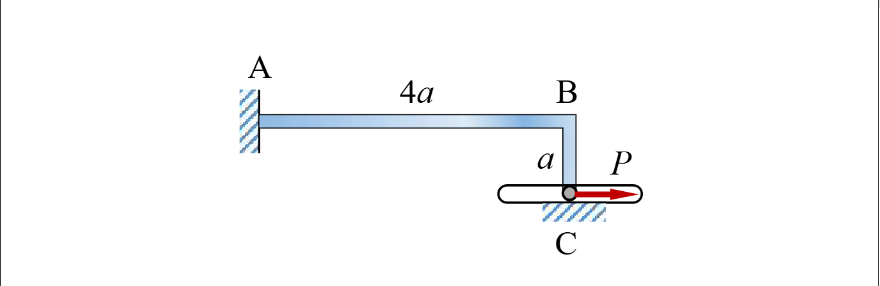
\includegraphics[width = 0.5\columnwidth]{figs/fig4.11.png}
    \caption*{}
    \label{fig:Q38}
    \end{figure}
    \hfill{(GATE ME 2022)}
\begin{enumerate}
    \item 3P/8, and downwards
\item 5P/8, and upwards
\item P/4, and downwards
\item 3P/4, and upwards
\end{enumerate}

\item A planar four-bar linkage mechanism with 3 revolute kinematic pairs and 1 prismatic kinematic pair is shown in the figure, where AB $\perp CE and FD \perp CE$. The T-shaped link CDEF is constructed such that the slider B can cross the point D, and CE is sufficiently long. For the given lengths as shown, the mechanism is 
    \begin{figure}[H]
    \centering
    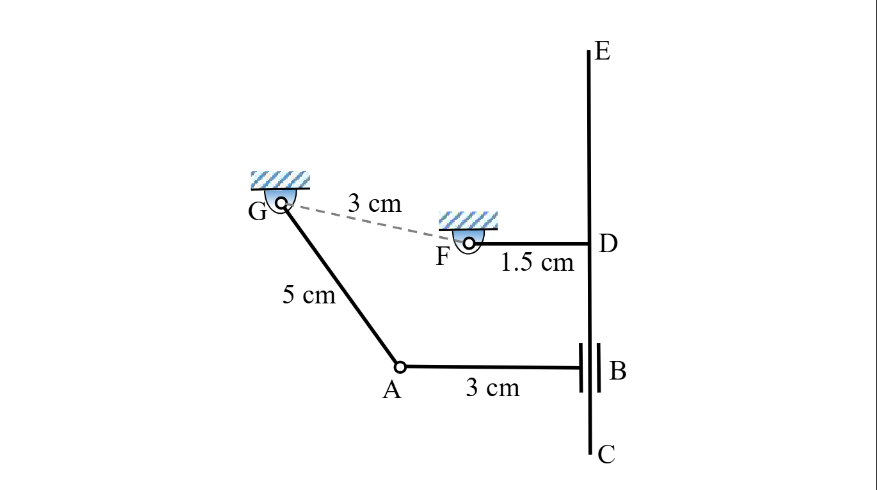
\includegraphics[width = 0.5\columnwidth]{figs/fig4.12.png}
    \caption*{}
    \label{fig:Q38}
    \end{figure}
    \hfill{(GATE ME 2022)}
\begin{enumerate}
  
\item a Grashof chain with links AG, AB, and CDEF completely rotatable about the ground link FG
\item a non-Grashof chain with all oscillating links 
\item a Grashof chain with AB completely rotatable about the ground link FG, and oscillatory links AG and CDEF
\item on the border of grashofer chains and ungrashfoer chains with uncertain figures
\end{enumerate}
\item Consider a forced single degree-of-freedom system governed by
\begin{align*}
\ddot{x}(t) + 2\zeta \omega_n \dot{x}(t) + \omega_n^2 x(t) = \omega_n^2 \cos(\omega t),
\end{align*}
where $\zeta$ and $\omega_n$ are the damping ratio and undamped natural frequency of the system, respectively, while $\omega$ is the forcing frequency.

The amplitude of the forced steady-state response of this system is given by
\[
\left[(1 - r^2)^2 + (2\zeta r)^2 \right]^{-1/2}, \quad \text{where } r = \omega/\omega_n.
\]
The peak amplitude of this response occurs at a frequency $\omega = \omega_p$.

If $\omega_d$ denotes the damped natural frequency of this system, which one of the following options is true?
\hfill{(GATE ME 2022)}
\begin{enumerate}
  
    \item $\omega_p < \omega_d < \omega_n$
    \item $\omega_p = \omega_d < \omega_n$
    \item $\omega_d < \omega_n = \omega_p$
    \item $\omega_d < \omega_n < \omega_p$
\end{enumerate}

\item A bracket is attached to a vertical column by means of two identical rivets U and V separated by a distance of 2a = 100 mm, as shown in the figure. The permissible shear stress of the rivet material is 50 MPa. If a load P = 10 kN is applied at an eccentricity e = 3$\sqrt{7} a$, the minimum cross-sectional area of each of the rivets to
mm2. avoid failure is
 \begin{figure}[H]
    \centering
    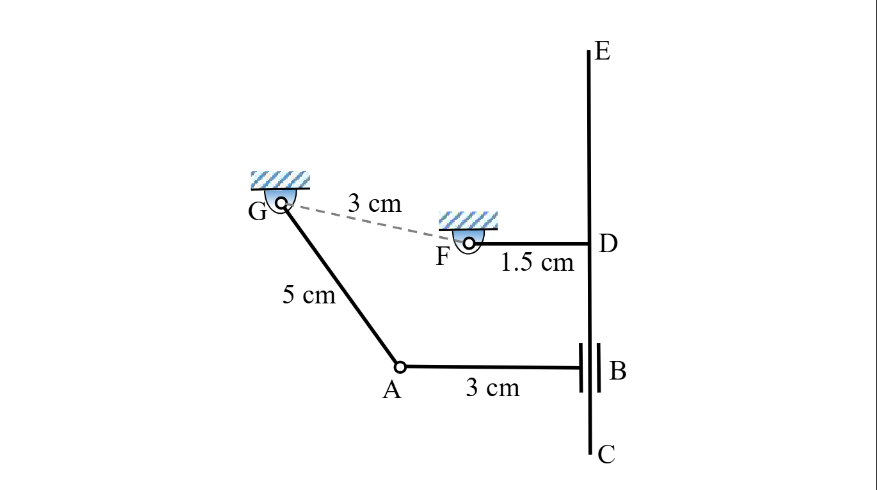
\includegraphics[width = 0.5\columnwidth]{figs/fig4.12.png}
    \caption*{}
    \label{fig:Q40}
    \end{figure}
    \hfill{(GATE ME 2022)}
    \begin{multicols}{4}
        \begin{enumerate}
            \item 800
            \item 25
            \item $100\sqrt{7}$
\item 200

        \end{enumerate}
    \end{multicols}
    \item In Fe--Fe$_3$C phase diagram, the eutectoid composition is 0.8 weight \% of carbon at 725~\textdegree C. The maximum solubility of carbon in $\alpha$-ferrite phase is 0.025 weight \% of carbon. A steel sample, having no other alloying element except 0.5 weight \% of carbon, is slowly cooled from 1000~\textdegree C to room temperature. The fraction of pro-eutectoid $\alpha$-ferrite in the above steel sample at room temperature is
\hfill{(GATE ME 2022)}
    \begin{multicols}{4}
    \begin{enumerate}
    \item 0.387
    \item 0.864
    \item 0.475
    \item 0.775
\end{enumerate}
    \end{multicols}
 \item \begin{align*}
\text{Activities A to K are required to complete a project. The time estimates and the} \\
\text{immediate predecessors of these activities are given in the table. If the project is to be} \\
\text{completed in the minimum possible time, the latest finish time for the activity G is} \\
\text{\underline{\hspace{3cm}} hours.}
\end{align*}

\begin{center}
\begin{tabular}{|>{\bfseries}c|c|c|}
\hline
Activity & Time (hours) & Immediate predecessors \\
\hline
A & 2 & -- \\
B & 3 & -- \\
C & 2 & -- \\
D & 4 & A \\
E & 5 & B \\
F & 4 & B \\
G & 3 & C \\
H & 10 & D, E \\
I & 5 & F \\
J & 8 & G \\
K & 3 & H, I, J \\
\hline
\end{tabular}
\end{center}
\hfill{(GATE ME 2022)}
 \begin{multicols}{4}
     \begin{enumerate}
         \item 5
         \item 10
         \item 8
         \item 9
     \end{enumerate}
 \end{multicols}
 \item 
 \begin{align*}
\text{A solid spherical bead of lead (uniform density } = 11000~\text{kg/m}^3) \text{ of diameter } \\
d = 0.1~\text{mm} \text{ sinks with a constant velocity } V \text{ in a large stagnant pool of a liquid} \\
\text{(dynamic viscosity } = 1.1 \times 10^{-3}~\text{kg} \cdot \text{m}^{-1} \cdot \text{s}^{-1}). \text{ The coefficient of drag is given by} \\
c_D = \frac{24}{\text{Re}}, \quad \text{where the Reynolds number (Re) is defined on the basis of the diameter} \\
\text{of the bead. The drag force acting on the bead is expressed as} \\
D = (c_D)\left(0.5 \rho V^2\right)\left(\frac{\pi d^2}{4}\right), \quad \text{where } \rho \text{ is the density of the liquid. Neglect the} \\
\text{buoyancy force. Using } g = 10~\text{m/s}^2, \text{ the velocity } V \text{ is } \underline{\hspace{2cm}} \text{ m/s}.
\end{align*}
\hfill{(GATE ME 2022)}
\begin{enumerate}
    
    \item $\dfrac{1}{24}$
    
    \item $\dfrac{1}{6}$
    
    \item $\dfrac{1}{18}$
    
    \item $\dfrac{1}{12}$
\end{enumerate}
\item Consider steady, one-dimensional compressible flow of a gas in a pipe of diameter 1 m. At one location in the pipe, the density and velocity are 1 kg/m3 and 100 m/s, respectively. At a downstream location in the pipe, the velocity is 170 m/s. If the pressure drop between these two locations is 10 kPa, the force exerted by the gas
on the pipe between these two locations is
\hfill{(GATE ME 2022)}
\begin{multicols}{4}
\begin{enumerate}
    \item $350\pi^2$
    \item $750\pi$
    \item $1000\pi$
    \item 3000
\end{enumerate}.
\end{multicols}
\item Consider a rod of uniform thermal conductivity whose one end (\(x = 0\)) is insulated and the other end (\(x = L\)) is exposed to flow of air at temperature \(T_{\infty}\) with convective heat transfer coefficient \(h\). The cylindrical surface of the rod is insulated so that the heat transfer is strictly along the axis of the rod. The rate of internal heat generation per unit volume inside the rod is given as:

\begin{align}
    \dot{q} = \cos\left(\frac{2\pi x}{L} \right)
\end{align}

The steady state temperature at the mid-location of the rod is given as \(T_A\). What will be the temperature at the same location, if the convective heat transfer coefficient increases to \(2h\)?
\hfill{(GATE ME 2022)}
\begin{enumerate}
    
 \item  $T_A + \frac{\dot{q}L}{2h} $
     \item $ 2T_A$ 
    \item $ T_A $
    \item $ T_A \left(1 - \frac{\dot{q}L}{4\pi h} \right) + \frac{\dot{q}L}{4\pi h} T_{\infty} $
\end{enumerate}

\item The system of linear equations in real \((x, y)\) given by

\begin{align}
    (x \quad y)
    \begin{bmatrix}
        2 & 5 - 2\alpha \\
        \alpha & 1
    \end{bmatrix}
    = (0 \quad 0)
\end{align}

involves a real parameter \(\alpha\) and has infinitely many non-trivial solutions for special value(s) of \(\alpha\). Which one or more among the following options is/are non-trivial solution(s) of \brak{x, y} for such special value(s) of \(\alpha\)?
\hfill{(GATE ME 2022)}
\begin{enumerate}
    
    \item  x=2,y=-2
    \item x=-1,y=4
    \item x=1,y=1
    \item x=4,y=-2
\end{enumerate}

 \item 

Let a random variable \(X\) follow Poisson distribution such that

\begin{align}
    \text{Prob}(X = 1) &= \text{Prob}(X = 2)
\end{align}

The value of \(\text{Prob}(X = 3)\) is  \textit{(round off to 2 decimal places).}
\hfill{(GATE ME 2022)}
\item Consider two vectors:
  \[
\vec{a} = 5\mathbf{i} + 7\mathbf{j} + 2\mathbf{k}
\]
\[
\vec{b} = 3\mathbf{i} - \mathbf{j} + 6\mathbf{k}
\]

Magnitude of the component of d orthogonal to b in the plane containing the vectors Bar{a} and Bar{b}is
(round off to 2 decimal places).
\hfill{(GATE ME 2022)}
\item 
A structure, along with the loads applied on it, is shown in the figure. Self-weight of all the members is negligible and all the pin joints are friction-less. AE is a single member that contains pin C. Likewise, BE is a single member that contains pin D. Members GI and FH are overlapping rigid members. The magnitude of the force
carried by member CI is kN (in integer).

 \begin{figure}[H]
    \centering
    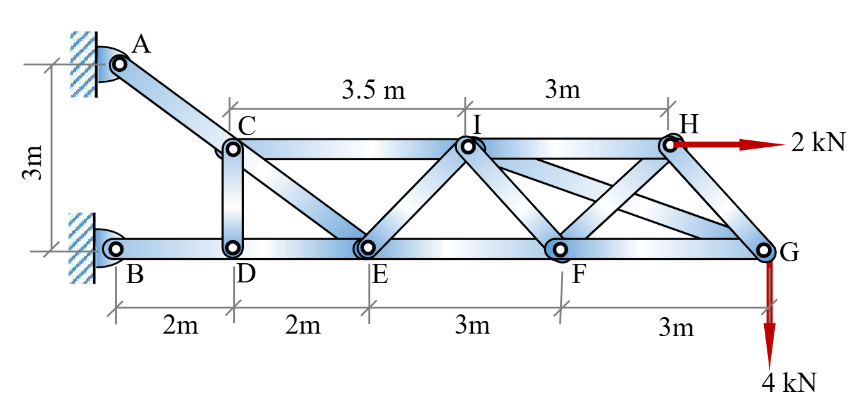
\includegraphics[width = 0.5\columnwidth]{figs/fig4.14.png}
    \caption*{}
    \label{fig:Q49}
    \end{figure}
\hfill{(GATE ME 2022)}
\item Two rigid massless rods PR and RQ are joined at frictionless pin-joint R and are resting on ground at P and Q, respectively, as shown in the figure. A vertical force  F acts on the pin R as shown. When the included angle $\theta$ < 90°, the rods remain in static equilibrium due to Coulomb friction between the rods and ground at locations P and Q. At $\theta$ = 90°, impending slip occurs simultaneously at points P and Q. Then the ratio of the coefficient of friction at Q to that at P $(\\frac{\mu_Q}{\mu_P}
)$ is  
( round off to two decimal places).
\begin{figure}[H]
    \centering
    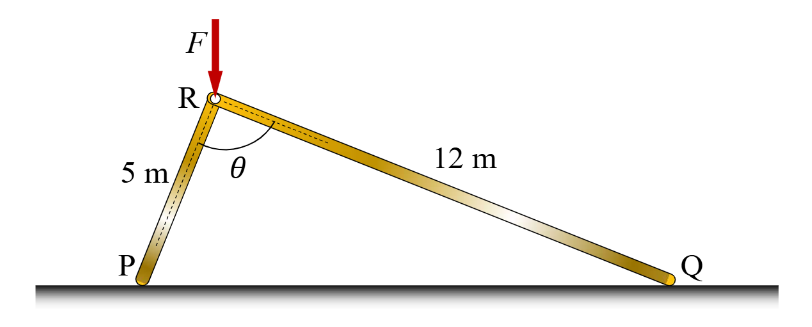
\includegraphics[width = 0.5\columnwidth]{figs/fig4.15.png}
    \caption*{}
    \label{fig:Q50}
    \end{figure}
\hfill{(GATE ME 2022)}
 \item A cylindrical disc of mass m = 1 kg and radius r = 0.15 m was spinning at $\omega = 5 rad/s $ when it was placed on a flat horizontal surface and released (refer to the figure). Gravity g acts vertically downwards as shown in the figure. The
coefficient of friction between the disc and the surface is finite and positive.Disregarding any other dissipation except that due to friction between the disc and the surface, the horizontal velocity of the center of the disc, when it starts rolling without slipping, will be $m/s$ (round off to 2 decimal places).

\begin{figure}[H]
    \centering
    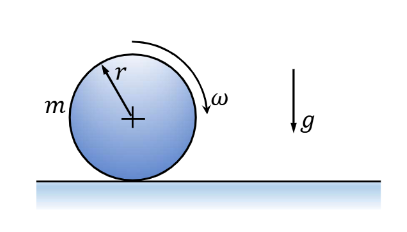
\includegraphics[width = 0.5\columnwidth]{figs/fig4.16.png}
    \caption*{}
    \label{fig:Q51}
    \end{figure}
\hfill{(GATE ME 2022)}
\item A thin-walled cylindrical pressure vessel has mean wall thickness of t and nominal radius of r. The Poisson's ratio of the wall material is 1/3. When it was subjected to some internal pressure, its nominal perimeter in the cylindrical portion increased
by 0.1 \% and the corresponding wall thickness became t. The corresponding change in the wall thickness of the cylindrical portion, i.e. 100 $\times \frac{\bar{t} - t}{t}$  is  \%
(round off to 3 decimal places).
\hfill{(GATE ME 2022)}
\item A schematic of an epicyclic gear train is shown in the figure. The sun ${gear 1}$ and planet  ${gear 2}$ are external, and the ring gear ${gear 3}$ is internal. Gear 1, gear 3 and arm OP are pivoted to the ground at O. Gear 2 is carried on the arm OP via the pivot
joint at P, and is in mesh with the other two gears. Gear 2 has 20 teeth and gear 3 has 80 teeth. If gear 1 is kept fixed at 0 rpm and gear 3 rotates at 900 rpm counter clockwise ${CCW}$, the magnitude of angular velocity of arm OP is(in integer).
\begin{figure}[H]
    \centering
    \includegraphics[width = 0.5\columnwidth]{figs/fig4.17.png}
    \caption*{}
    \label{fig:Q52}
    \end{figure}
    \hfill{(GATE ME 2022)}
 \item Under orthogonal cutting condition, a turning operation is carried out on a metallic workpiece at a cutting speed of 4 m/s. The orthogonal rake angle of the cutting tool is 5\degree. The uncut chip thickness and width of cut are 0.2 mm and 3 mm,respectively. In this turning operation, the resulting friction angle and shear angle
are 45\degree and 25\degree, respectively. If the dynamic yield shear strength of the workpiece material under this cutting condition is 1000 MPa, then the cutting force is N (round off to one decimal place).

\item 
A 1 mm thick cylindrical tube, 100 mm in diameter, is orthogonally turned such that the entire wall thickness of the tube is cut in a single pass. The axial feed of the tool is 1 m/minute and the specific cutting energy $\brak{u}$ of the tube material is
carry out this operation is 6 $J/mm^3$ Neglect contribution of feed force towards power. The power required to kW (round off to one decimal place).
\hfill{(GATE ME 2022)}
 
\item A 4 mm thick aluminum sheet of width \( w = 100 \) mm is rolled in a two-roll mill of roll diameter 200 mm each. The workpiece is lubricated with a mineral oil, which gives a coefficient of friction, \( \mu = 0.1 \). The flow stress (\( \sigma \)) of the material in MPa is
    \begin{align*}
        \sigma = 207 + 414 \varepsilon,
    \end{align*}

    where \( \varepsilon \) is the true strain.
Assuming rolling to be a plane strain deformation process, the roll separation force \( F \) for maximum permissible draft (thickness reduction) is \underline{\hspace{3cm}} kN \textit{(round off to the nearest integer)}.
    \textbf{Use:}
    \begin{align*}
        F = 1.15 \, \bar{\sigma} \left( 1 + \frac{\mu L}{2\bar{h}} \right) wL,
    \end{align*}
    where:
        \( \bar{\sigma} \): average flow stress
         \( L \): roll-workpiece contact length
         \( \bar{h} \): average sheet thickness
         \hfill{(GATE ME 2022)}
\item Two mild steel plates of similar thickness, in butt-joint configuration, are welded by gas tungsten arc welding process using the following welding parameters:
 \begin{center}
\begin{tabular}{|l|c|}
        \hline
        \textbf{Welding voltage} & 20 V \\
        \hline
        \textbf{Welding current} & 150 A \\
        \hline
        \textbf{Welding speed}   & 5 mm/s \\
        \hline
    \end{tabular}
    \end{center}
 A filler wire of the same mild steel material having 3 mm diameter is used in this welding process. The filler wire feed rate is selected such that the final weld bead is composed of 60\% volume of filler and 40\% volume of plate material.
The heat required to melt the mild steel material is:
$10 \, \text{J/mm}^3$
 The heat transfer factor is \( 0.7 \) and the melting factor is \( 0.6 \). The feed rate of the filler wire is \underline{\hspace{2cm}} mm/s \textit{(round off to one decimal place)}.
\hfill{(GATE ME 2022)}
\item An assignment problem is solved to minimize the total processing time of four jobs $\brak{1,2,3 and 4}$ on four different machines such that each job is processed exactly by one machine and each machine processes exactly one job. The minimum total
processing time is found to be 500 minutes. Due to a change in design, the processing time of Job 4 on each machine has increased by 20 minutes. The revised minimum total processing  time will be 
\hfill{(GATE ME 2022)}
\item The product structure diagram shows the number of different components required at each level to produce one unit of the final product P. If there are 50 units of on-hand inventory of component A, the number of additional units of component A needed to produce 10 units of product P is(in integer).
 \begin{figure}[H]
    \centering
    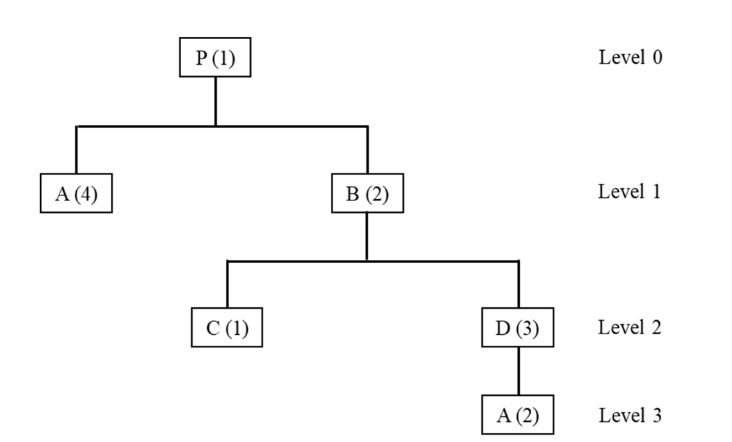
\includegraphics[width = 0.5\columnwidth]{figs/fig4.18.png}
    \caption*{}
    \label{fig:Q59}
    \end{figure}
\hfill{(GATE ME 2022)}
 \item Consider a one-dimensional steady heat conduction process through a solid slab of thickness 0.1 m. The higher temperature side A has a surface temperature of 80 $\degree C$, and the heat transfer rate per unit area to low temperature side B is 4.5 $kW/m_2$. The thermal conductivity of the slab is 15 W/m.K. The rate of entropy generation per unit area during the heat transfer process is $W/m^2/K$ (round off to 2 decimal process)

\hfill{(GATE ME 2022)}
\item 
In a steam power plant based on Rankine cycle, steam is initially expanded in a high-pressure turbine. The steam is then reheated in a reheater and finally expanded in a low-pressure turbine. The expansion work in the high-pressure turbine is 400 kJ/kg and in the low-pressure turbine is 850 kJ/kg, whereas the pump work is 15 kJ/kg. If the cycle efficiency is 32 \%, the heat rejected in the condenser
kJ/kg (round off to 2 decimal places).
\hfill{(GATE ME 2022)}
\item 
An engine running on an air standard Otto cycle has a displacement volume $250 cm^3$ and a clearance volume 35.7 $cm^3$. The pressure and temperature at the beginning of the compression process are 100 kPa and 300 K, respectively. Heat transfer during constant-volume heat addition process is 800 kJ/kg. The specific heat at constant volume is 0.718 kJ/kg.K and the ratio of specific heats at constant
pressure and constant volume is 1.4. Assume the specific heats to remain constant during the cycle. The maximum pressure in the cycle is
kPa (round off to the nearest integer).
\hfill{(GATE ME 2022)}

\item A steady two-dimensional flow field is specified by the stream function
$\psi = kx^3 y$,
where \( x \) and \( y \) are in meter and the constant \( k = 1 \, \text{m}^{-2}\text{s}^{-1} \). The magnitude of acceleration at a point \( (x, y) = (1\, \text{m}, 1\, \text{m}) \) is \underline{\hspace{2cm}} m/s\(^2\) \textit{(round off to 2 decimal places)}.
\hfill{(GATE ME 2022)}
\item Consider a solid slab (thermal conductivity, \( k = 10 \, \text{W}\cdot\text{m}^{-1}\cdot\text{K}^{-1} \)) with thickness \( 0.2 \, \text{m} \) and of infinite extent in the other two directions as shown in the figure. Surface \textbf{2}, at 300 K, is exposed to a fluid flow at a free stream temperature (\( T_{\infty} \)) of 293 K, with a convective heat transfer coefficient (\( h \)) of \( 100 \, \text{W}\cdot\text{m}^{-2}\cdot\text{K}^{-1} \). 

Surface \textbf{2} is opaque, diffuse and gray with an emissivity (\( \varepsilon \)) of 0.5 and exchanges heat by radiation with very large surroundings at 0 K. Radiative heat transfer inside the solid slab is neglected. The Stefan-Boltzmann constant is 
\[
\sigma = 5.67 \times 10^{-8} \, \text{W}\cdot\text{m}^{-2}\cdot\text{K}^{-4}.
\]

The temperature \( T_1 \) of Surface \textbf{1} of the slab, under steady-state conditions, is \underline{\hspace{2cm}} K \textit{(round off to the nearest integer)}.
\begin{figure}[H]
    \centering
    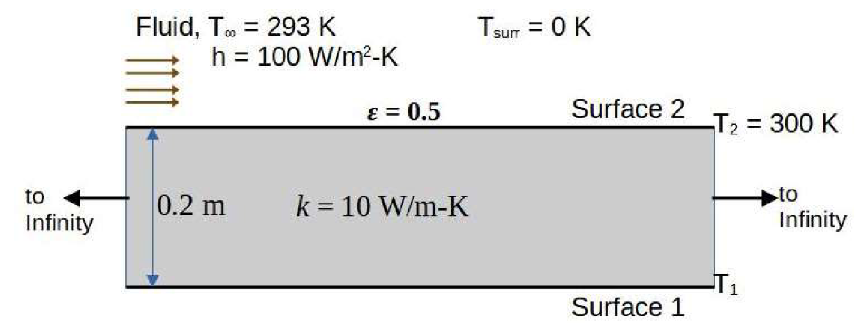
\includegraphics[width = 0.5\columnwidth]{figs/fig4.19.png}
    \caption*{}
    \label{fig:Q64}
    \end{figure}
\hfill{(GATE ME 2022)}

 \item During open heart surgery, a patients blood is cooled down to $25 \degree C $ 
from $37 \degree C$ using a concentric tube counter flow heat exchanger. 
Water enters the heat exchanger at $4 \degree C$ and leaves at $18 \degree C $. 
Blood flow rate during the surgery is
Use the following fluid properties:

\begin{center}
\begin{tabular}{|l|c|c|}
\hline
\textbf{Fluid} & \textbf{Density (kg/m\(^3\))} & \textbf{Specific heat (J/kg-K)} \\
\hline
Blood & 1050 & 3740 \\
\hline
Water & 1000 & 4200 \\
\hline
\end{tabular}
\end{center}
 
Effectiveness of the heat exchanger is \underline{\hspace{2cm}} \textit{(round off to 2 decimal places)}.

\hfill{(GATE ME 2022)}
\end{enumerate}
\end{document}